\documentclass[12pt,a4paper]{article}

% ===== PACKAGES =====
\usepackage[utf8]{inputenc}
\usepackage[T1]{fontenc}
\usepackage{amsmath,amssymb,amsfonts}
\usepackage{graphicx}
\usepackage[margin=1in]{geometry}
\usepackage{hyperref}
\usepackage{xcolor}
\usepackage{tikz}
\usepackage{circuitikz}
\usepackage{booktabs}
\usepackage{multirow}
\usepackage{array}
\usepackage{enumitem}
\usepackage{fancyhdr}
\usepackage{tcolorbox}
\usepackage{float}

% TikZ Libraries for FSM diagrams
\usetikzlibrary{automata,positioning,arrows.meta,shapes.geometric,calc,decorations.pathreplacing}

% ===== CUSTOM COLORS =====
\definecolor{statecolor}{RGB}{66,133,244}
\definecolor{transcolor}{RGB}{52,168,83}
\definecolor{acceptcolor}{RGB}{234,67,53}
\definecolor{headerblue}{RGB}{26,115,232}
\definecolor{lightgray}{RGB}{245,245,245}

% ===== CUSTOM STYLES =====
\tcbuselibrary{skins,breakable}

\newtcolorbox{solutionbox}[1][]{
  colback=blue!5!white,
  colframe=headerblue,
  fonttitle=\bfseries,
  title=#1,
  breakable
}

\newtcolorbox{conceptbox}[1][]{
  colback=green!5!white,
  colframe=green!50!black,
  fonttitle=\bfseries,
  title=#1,
  breakable
}

\newtcolorbox{warningbox}[1][]{
  colback=red!5!white,
  colframe=red!50!black,
  fonttitle=\bfseries,
  title=#1
}

% ===== FSM DIAGRAM STYLES (COMPACT) =====
\tikzset{
  fsm state/.style={
    circle,
    draw=statecolor,
    fill=statecolor!15,
    thick,
    minimum size=0.8cm,
    inner sep=1pt,
    font=\scriptsize\bfseries
  },
  fsm init/.style={
    fsm state,
    fill=green!15,
    draw=green!60!black
  },
  fsm accept/.style={
    fsm state,
    fill=acceptcolor!15,
    draw=acceptcolor
  },
  arrow/.style={
    ->,
    >=Stealth,
    thick,
    font=\tiny
  },
  every edge/.style={draw, arrow}
}

% ===== HEADER/FOOTER =====
\pagestyle{fancy}
\fancyhf{}
\fancyhead[L]{\textcolor{headerblue}{\textbf{DSD Assignment 1 - Solutions}}}
\fancyhead[R]{\textcolor{headerblue}{Spring 2026}}
\fancyfoot[C]{\thepage}
\renewcommand{\headrulewidth}{2pt}
\renewcommand{\headrule}{\hbox to\headwidth{\color{headerblue}\leaders\hrule height \headrulewidth\hfill}}

% ===== DOCUMENT =====
\begin{document}

% ===== TITLE PAGE =====
\begin{titlepage}
\centering
\vspace*{2cm}

{\Huge\bfseries\textcolor{headerblue}{Digital System Design}}\\[0.5cm]
{\LARGE Assignment 1 - Complete Solutions}\\[2cm]

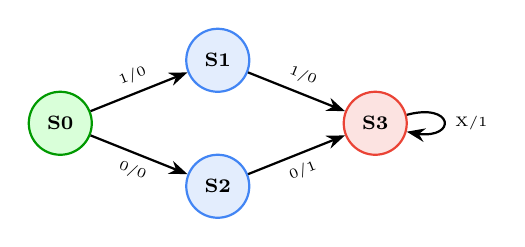
\begin{tikzpicture}[scale=0.8]
  % Decorative FSM illustration
  \node[fsm init] (s0) at (0,0) {S0};
  \node[fsm state] (s1) at (2.5,1) {S1};
  \node[fsm state] (s2) at (2.5,-1) {S2};
  \node[fsm accept] (s3) at (5,0) {S3};

  \draw[arrow] (s0) -- node[above,sloped] {\tiny 1/0} (s1);
  \draw[arrow] (s0) -- node[below,sloped] {\tiny 0/0} (s2);
  \draw[arrow] (s1) -- node[above,sloped] {\tiny 1/0} (s3);
  \draw[arrow] (s2) -- node[below,sloped] {\tiny 0/1} (s3);
  \draw[arrow] (s3) to[loop right] node[right] {\tiny X/1} (s3);
\end{tikzpicture}

\vspace{2cm}

\begin{tabular}{rl}
\textbf{Course:} & Digital System Design (Theory)\\[0.3cm]
\textbf{Reference:} & Digital Design, First Edition\\
& by Frank Vahid (Wiley, 2007)\\
& Chapters 2, 3, and 4\\[0.3cm]
\textbf{Topics:} & Combinational Logic Design\\
& Finite State Machines\\
& Sequential Circuit Design
\end{tabular}

\vfill

{\large Prepared: \today}

\end{titlepage}

% ===== TABLE OF CONTENTS =====
\tableofcontents
\newpage

% =========================================================================
% PART I: CHAPTER SUMMARIES
% =========================================================================
\part{Theoretical Foundation}
\section{Chapter 2: Combinational Logic Design}

\begin{conceptbox}[Key Concepts - Combinational Circuits]
Combinational circuits are digital circuits where outputs depend \textbf{only} on current inputs (no memory). The design process follows a structured approach from problem specification to gate implementation.
\end{conceptbox}

\subsection{The Combinational Design Process}

\begin{enumerate}[label=\textbf{Step \arabic*:}]
  \item \textbf{Capture the Function} - Create a truth table or Boolean equations
  \item \textbf{Convert to Equations} - Derive Sum-of-Products (SOP) or Product-of-Sums (POS)
  \item \textbf{Minimize} - Use K-maps or algebraic methods
  \item \textbf{Implement} - Draw the circuit using gates
\end{enumerate}

\subsection{Decoders}

\begin{conceptbox}[Decoder Definition]
A \textbf{decoder} is a combinational circuit that converts an $n$-bit binary input into $2^n$ output lines, where exactly one output is active at a time.
\end{conceptbox}

\subsubsection{2-to-4 Decoder with Enable}

\begin{figure}[H]
\centering
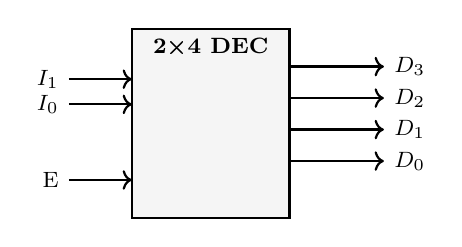
\begin{tikzpicture}[scale=0.8]
  % Decoder block
  \draw[thick, fill=lightgray] (0,0) rectangle (2.5,3);
  \node at (1.25,2.7) {\footnotesize\textbf{2×4 DEC}};

  % Inputs
  \draw[thick, ->] (-1,2.2) -- (0,2.2) node[pos=0, left] {\footnotesize $I_1$};
  \draw[thick, ->] (-1,1.8) -- (0,1.8) node[pos=0, left] {\footnotesize $I_0$};
  \draw[thick, ->] (-1,0.6) -- (0,0.6) node[pos=0, left] {\footnotesize E};

  % Outputs
  \draw[thick, ->] (2.5,2.4) -- (4,2.4) node[right] {\footnotesize $D_3$};
  \draw[thick, ->] (2.5,1.9) -- (4,1.9) node[right] {\footnotesize $D_2$};
  \draw[thick, ->] (2.5,1.4) -- (4,1.4) node[right] {\footnotesize $D_1$};
  \draw[thick, ->] (2.5,0.9) -- (4,0.9) node[right] {\footnotesize $D_0$};
\end{tikzpicture}
\caption{2×4 Decoder with Enable Input}
\end{figure}

\subsubsection{Truth Table for 2×4 Decoder}

\begin{table}[H]
\centering
\begin{tabular}{ccc|cccc}
\toprule
\textbf{E} & \textbf{$I_1$} & \textbf{$I_0$} & \textbf{$D_0$} & \textbf{$D_1$} & \textbf{$D_2$} & \textbf{$D_3$} \\
\midrule
0 & X & X & 0 & 0 & 0 & 0 \\
1 & 0 & 0 & 1 & 0 & 0 & 0 \\
1 & 0 & 1 & 0 & 1 & 0 & 0 \\
1 & 1 & 0 & 0 & 0 & 1 & 0 \\
1 & 1 & 1 & 0 & 0 & 0 & 1 \\
\bottomrule
\end{tabular}
\caption{2×4 Decoder Truth Table}
\end{table}

\subsection{Multiplexers}

A \textbf{multiplexer (MUX)} selects one of $2^n$ data inputs based on $n$ select lines.

\begin{figure}[H]
\centering
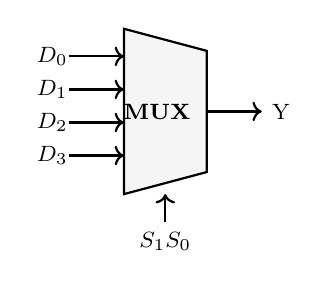
\begin{tikzpicture}[scale=0.7]
  % MUX trapezoid
  \draw[thick, fill=lightgray] (0,0) -- (0,3) -- (1.5,2.6) -- (1.5,0.4) -- cycle;
  \node at (0.6,1.5) {\footnotesize\textbf{MUX}};

  % Data inputs
  \foreach \i/\y in {0/2.5, 1/1.9, 2/1.3, 3/0.7} {
    \draw[thick, ->] (-1,\y) -- (0,\y);
    \node at (-1.3,\y) {\footnotesize $D_\i$};
  }

  % Select inputs
  \draw[thick, ->] (0.75,-0.5) -- (0.75,0) node[pos=0, below] {\footnotesize $S_1S_0$};

  % Output
  \draw[thick, ->] (1.5,1.5) -- (2.5,1.5) node[right] {\footnotesize Y};
\end{tikzpicture}
\caption{4-to-1 Multiplexer Symbol}
\end{figure}

\newpage
\section{Chapter 3: Sequential Logic Design - Controllers}

\begin{conceptbox}[Key Concepts - Sequential Circuits]
Sequential circuits have \textbf{memory} - outputs depend on both current inputs AND past inputs (stored state). The fundamental building block is the flip-flop.
\end{conceptbox}

\subsection{Finite State Machines (FSMs)}

An FSM is defined by the 5-tuple: $(Q, \Sigma, \delta, q_0, F)$

\begin{itemize}
  \item $Q$ = Finite set of states
  \item $\Sigma$ = Input alphabet
  \item $\delta$ = Transition function: $Q \times \Sigma \rightarrow Q$
  \item $q_0$ = Initial state
  \item $F$ = Set of final/accepting states
\end{itemize}

\subsection{FSM Types}

\begin{table}[H]
\centering
\begin{tabular}{lll}
\toprule
\textbf{Type} & \textbf{Output Depends On} & \textbf{Output Timing} \\
\midrule
\textbf{Moore Machine} & Current state only & Output with state \\
\textbf{Mealy Machine} & Current state + input & Output with transition \\
\bottomrule
\end{tabular}
\caption{Comparison of Moore and Mealy FSMs}
\end{table}

\subsection{FSM Design Process}

\begin{enumerate}[label=\textbf{Step \arabic*:}]
  \item \textbf{Understand the Problem} - Identify inputs, outputs, and behavior
  \item \textbf{Draw State Diagram} - Create states and transitions
  \item \textbf{Create State Table} - List all state transitions
  \item \textbf{Assign State Encoding} - Binary codes to states
  \item \textbf{Derive Next-State Logic} - Boolean equations for flip-flops
  \item \textbf{Derive Output Logic} - Boolean equations for outputs
  \item \textbf{Implement} - Draw circuit with flip-flops and gates
\end{enumerate}

\subsection{State Diagram Notation}

\begin{figure}[H]
\centering
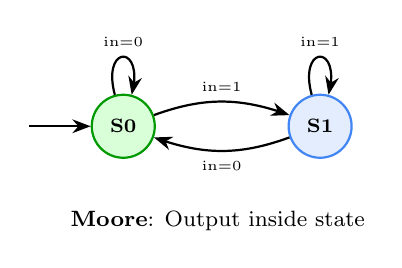
\begin{tikzpicture}[node distance=2.5cm]
  % Moore Machine Example
  \node[fsm init] (s0) {S0};
  \node[fsm state, right of=s0] (s1) {S1};

  \draw[arrow] (s0) to[bend left=20] node[above] {\tiny in=1} (s1);
  \draw[arrow] (s1) to[bend left=20] node[below] {\tiny in=0} (s0);
  \draw[arrow] (s0) to[loop above] node[above] {\tiny in=0} (s0);
  \draw[arrow] (s1) to[loop above] node[above] {\tiny in=1} (s1);

  % Initial arrow
  \draw[arrow] (-1.2,0) -- (s0);

  \node at (1.2,-1.2) {\footnotesize\textbf{Moore}: Output inside state};
\end{tikzpicture}
\hspace{1.5cm}
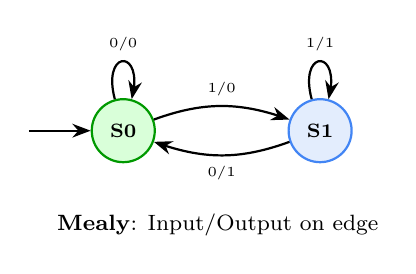
\begin{tikzpicture}[node distance=2.5cm]
  % Mealy Machine Example
  \node[fsm init] (s0) {S0};
  \node[fsm state, right of=s0] (s1) {S1};

  \draw[arrow] (s0) to[bend left=20] node[above] {\tiny 1/0} (s1);
  \draw[arrow] (s1) to[bend left=20] node[below] {\tiny 0/1} (s0);
  \draw[arrow] (s0) to[loop above] node[above] {\tiny 0/0} (s0);
  \draw[arrow] (s1) to[loop above] node[above] {\tiny 1/1} (s1);

  \draw[arrow] (-1.2,0) -- (s0);

  \node at (1.2,-1.2) {\footnotesize\textbf{Mealy}: Input/Output on edge};
\end{tikzpicture}
\caption{Moore vs Mealy Machine Notation}
\end{figure}

\newpage
\section{Chapter 4: Datapath Components}

\begin{conceptbox}[Key Concepts - Datapath]
Datapaths process multi-bit data using registers, ALUs, and interconnections. Controllers (FSMs) direct datapaths to perform operations.
\end{conceptbox}

\subsection{Registers and Counters}

\begin{figure}[H]
\centering
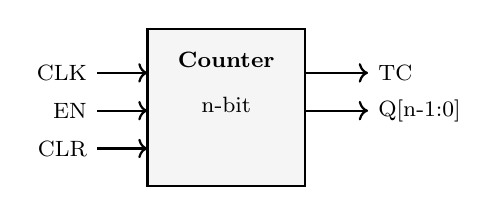
\begin{tikzpicture}[scale=0.8]
  % Counter block
  \draw[thick, fill=lightgray] (0,0) rectangle (2.5,2.5);
  \node at (1.25,2) {\footnotesize\textbf{Counter}};
  \node at (1.25,1.3) {\footnotesize n-bit};

  % Inputs
  \draw[thick, ->] (-0.8,1.8) -- (0,1.8) node[pos=0, left] {\footnotesize CLK};
  \draw[thick, ->] (-0.8,1.2) -- (0,1.2) node[pos=0, left] {\footnotesize EN};
  \draw[thick, ->] (-0.8,0.6) -- (0,0.6) node[pos=0, left] {\footnotesize CLR};

  % Output
  \draw[thick, ->] (2.5,1.2) -- (3.5,1.2) node[right] {\footnotesize Q[n-1:0]};
  \draw[thick, ->] (2.5,1.8) -- (3.5,1.8) node[right] {\footnotesize TC};
\end{tikzpicture}
\caption{n-bit Counter with Terminal Count Output}
\end{figure}

\subsection{Controller-Datapath Architecture}

\begin{figure}[H]
\centering
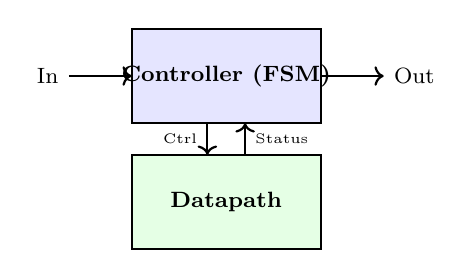
\begin{tikzpicture}[scale=0.8]
  % Controller
  \draw[thick, fill=blue!10] (0,2) rectangle (3,3.5);
  \node at (1.5,2.75) {\footnotesize\textbf{Controller (FSM)}};

  % Datapath
  \draw[thick, fill=green!10] (0,0) rectangle (3,1.5);
  \node at (1.5,0.75) {\footnotesize\textbf{Datapath}};

  % Connections
  \draw[thick, ->] (1.2,2) -- (1.2,1.5) node[midway, left] {\tiny Ctrl};
  \draw[thick, ->] (1.8,1.5) -- (1.8,2) node[midway, right] {\tiny Status};

  % External
  \draw[thick, ->] (-1,2.75) -- (0,2.75) node[pos=0, left] {\footnotesize In};
  \draw[thick, ->] (3,2.75) -- (4,2.75) node[right] {\footnotesize Out};
\end{tikzpicture}
\caption{Controller-Datapath Architecture}
\end{figure}

% =========================================================================
% PART II: ASSIGNMENT SOLUTIONS
% =========================================================================
\newpage
\part{Assignment Solutions}

% =========================================================================
% QUESTION 1
% =========================================================================
\section{Question 1: Fuel Sensor System (20 marks)}

\begin{solutionbox}[Problem Statement]
Design a combinational circuit for a fuel sensor system that detects fuel level using five sensors ($S_0$ to $S_4$). The output is a 3-bit binary representation of the fuel level. Use \textbf{five 2×4 decoders with enable inputs} and any additional logic gates.
\end{solutionbox}

\subsection{Understanding the Problem}

The fuel tank has 5 sensors positioned at different heights:
\begin{itemize}
  \item $S_0$ = Bottom sensor (covered first)
  \item $S_4$ = Top sensor (covered last)
  \item Sensor = 1 when covered by fuel
  \item Valid patterns: Contiguous 1s from bottom
\end{itemize}

\subsection{Truth Table}

\begin{table}[H]
\centering
\begin{tabular}{ccccc|ccc|c}
\toprule
\textbf{$S_4$} & \textbf{$S_3$} & \textbf{$S_2$} & \textbf{$S_1$} & \textbf{$S_0$} & \textbf{$F_2$} & \textbf{$F_1$} & \textbf{$F_0$} & \textbf{Level} \\
\midrule
0 & 0 & 0 & 0 & 0 & 0 & 0 & 0 & Empty (0) \\
0 & 0 & 0 & 0 & 1 & 0 & 0 & 1 & Level 1 \\
0 & 0 & 0 & 1 & 1 & 0 & 1 & 0 & Level 2 \\
0 & 0 & 1 & 1 & 1 & 0 & 1 & 1 & Level 3 \\
0 & 1 & 1 & 1 & 1 & 1 & 0 & 0 & Level 4 \\
1 & 1 & 1 & 1 & 1 & 1 & 0 & 1 & Full (5) \\
\bottomrule
\end{tabular}
\caption{Fuel Level Truth Table (Valid Patterns Only)}
\end{table}

\subsection{Design Approach Using 2×4 Decoders}

\begin{conceptbox}[Design Strategy]
We use five 2×4 decoders to detect specific fuel levels. Each decoder's enable is controlled by higher-level sensor conditions.
\end{conceptbox}

\subsection{Boolean Equations}

Level detection signals:
\begin{align}
L_0 &= \overline{S_4} \cdot \overline{S_3} \cdot \overline{S_2} \cdot \overline{S_1} \cdot \overline{S_0} \\
L_1 &= \overline{S_4} \cdot \overline{S_3} \cdot \overline{S_2} \cdot \overline{S_1} \cdot S_0 \\
L_2 &= \overline{S_4} \cdot \overline{S_3} \cdot \overline{S_2} \cdot S_1 \cdot S_0 \\
L_3 &= \overline{S_4} \cdot \overline{S_3} \cdot S_2 \cdot S_1 \cdot S_0 \\
L_4 &= \overline{S_4} \cdot S_3 \cdot S_2 \cdot S_1 \cdot S_0 \\
L_5 &= S_4 \cdot S_3 \cdot S_2 \cdot S_1 \cdot S_0
\end{align}

Final outputs (binary encoding):
\begin{align}
F_2 &= L_4 + L_5 \\
F_1 &= L_2 + L_3 \\
F_0 &= L_1 + L_3 + L_5
\end{align}

\subsection{Circuit Block Diagram}

\begin{figure}[H]
\centering
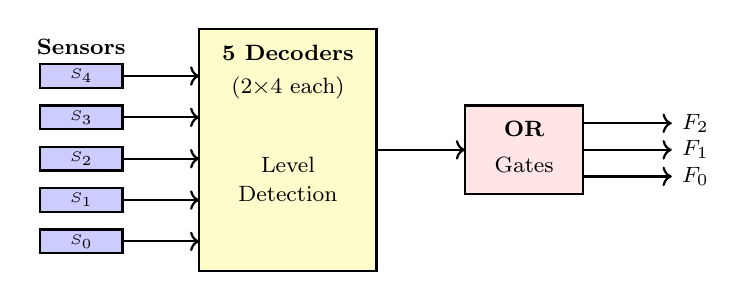
\begin{tikzpicture}[scale=0.75]

  % Sensors on left
  \node at (-3.5, 3.5) {\footnotesize\textbf{Sensors}};
  \foreach \i/\y in {4/3, 3/2.3, 2/1.6, 1/0.9, 0/0.2} {
    \draw[thick, fill=blue!20] (-4.2,\y-0.2) rectangle (-2.8, \y+0.2);
    \node at (-3.5, \y) {\tiny $S_\i$};
    \draw[thick, ->] (-2.8, \y) -- (-1.5, \y);
  }

  % Decoder Bank
  \draw[thick, fill=yellow!20] (-1.5, -0.3) rectangle (1.5, 3.8);
  \node at (0, 3.4) {\footnotesize\textbf{5 Decoders}};
  \node at (0, 2.8) {\footnotesize (2×4 each)};
  \node at (0, 1.5) {\footnotesize Level};
  \node at (0, 1) {\footnotesize Detection};

  % OR gates
  \draw[thick, fill=red!10] (3, 1) rectangle (5, 2.5);
  \node at (4, 2.1) {\footnotesize\textbf{OR}};
  \node at (4, 1.5) {\footnotesize Gates};

  % Connections
  \draw[thick, ->] (1.5, 1.75) -- (3, 1.75);

  % Final Outputs
  \draw[thick, ->] (5, 2.2) -- (6.5, 2.2) node[right] {\footnotesize $F_2$};
  \draw[thick, ->] (5, 1.75) -- (6.5, 1.75) node[right] {\footnotesize $F_1$};
  \draw[thick, ->] (5, 1.3) -- (6.5, 1.3) node[right] {\footnotesize $F_0$};

\end{tikzpicture}
\caption{Fuel Sensor System Block Diagram}
\end{figure}

\subsection{Detailed Decoder Connections}

\begin{figure}[H]
\centering
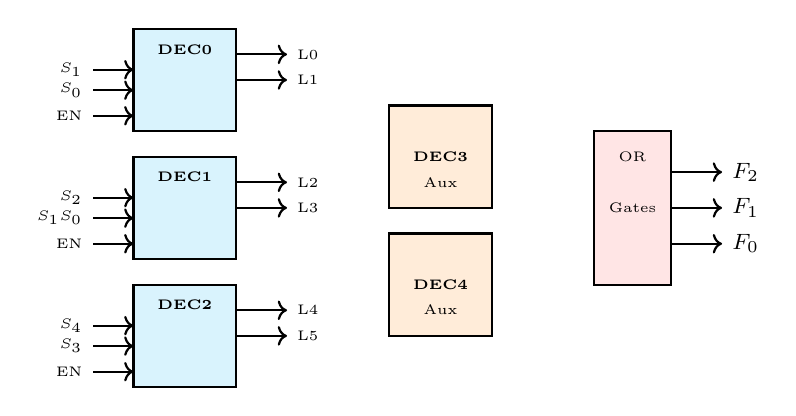
\begin{tikzpicture}[scale=0.65]

  % DEC 0
  \draw[thick, fill=cyan!15] (0,8) rectangle (2,10);
  \node at (1,9.6) {\tiny\textbf{DEC0}};
  \draw[thick, <-] (0,9.2) -- (-0.8,9.2) node[left] {\tiny $S_1$};
  \draw[thick, <-] (0,8.8) -- (-0.8,8.8) node[left] {\tiny $S_0$};
  \draw[thick, <-] (0,8.3) -- (-0.8,8.3) node[left] {\tiny EN};
  \draw[thick, ->] (2,9.5) -- (3,9.5) node[right] {\tiny L0};
  \draw[thick, ->] (2,9) -- (3,9) node[right] {\tiny L1};

  % DEC 1
  \draw[thick, fill=cyan!15] (0,5.5) rectangle (2,7.5);
  \node at (1,7.1) {\tiny\textbf{DEC1}};
  \draw[thick, <-] (0,6.7) -- (-0.8,6.7) node[left] {\tiny $S_2$};
  \draw[thick, <-] (0,6.3) -- (-0.8,6.3) node[left] {\tiny $S_1S_0$};
  \draw[thick, <-] (0,5.8) -- (-0.8,5.8) node[left] {\tiny EN};
  \draw[thick, ->] (2,7) -- (3,7) node[right] {\tiny L2};
  \draw[thick, ->] (2,6.5) -- (3,6.5) node[right] {\tiny L3};

  % DEC 2
  \draw[thick, fill=cyan!15] (0,3) rectangle (2,5);
  \node at (1,4.6) {\tiny\textbf{DEC2}};
  \draw[thick, <-] (0,4.2) -- (-0.8,4.2) node[left] {\tiny $S_4$};
  \draw[thick, <-] (0,3.8) -- (-0.8,3.8) node[left] {\tiny $S_3$};
  \draw[thick, <-] (0,3.3) -- (-0.8,3.3) node[left] {\tiny EN};
  \draw[thick, ->] (2,4.5) -- (3,4.5) node[right] {\tiny L4};
  \draw[thick, ->] (2,4) -- (3,4) node[right] {\tiny L5};

  % DEC 3 & 4 (auxiliary)
  \draw[thick, fill=orange!15] (5,6.5) rectangle (7,8.5);
  \node at (6,7.5) {\tiny\textbf{DEC3}};
  \node at (6,7) {\tiny Aux};

  \draw[thick, fill=orange!15] (5,4) rectangle (7,6);
  \node at (6,5) {\tiny\textbf{DEC4}};
  \node at (6,4.5) {\tiny Aux};

  % Output OR gates
  \draw[thick, fill=red!10] (9,5) rectangle (10.5,8);
  \node at (9.75,7.5) {\tiny OR};
  \node at (9.75,6.5) {\tiny Gates};

  % Final outputs
  \draw[thick, ->] (10.5,7.2) -- (11.5,7.2) node[right] {\footnotesize $F_2$};
  \draw[thick, ->] (10.5,6.5) -- (11.5,6.5) node[right] {\footnotesize $F_1$};
  \draw[thick, ->] (10.5,5.8) -- (11.5,5.8) node[right] {\footnotesize $F_0$};

\end{tikzpicture}
\caption{Five 2×4 Decoders Implementation}
\end{figure}

% =========================================================================
% QUESTION 2
% =========================================================================
\newpage
\section{Question 2: Photo Booth FSM (10 marks)}

\begin{solutionbox}[Problem Statement]
Design an FSM for a photo booth that accepts nickels (5¢), dimes (10¢), and quarters (25¢). Photo costs \textbf{25¢}. Return change if overpaid.
\end{solutionbox}

\subsection{Input/Output Definition}

\begin{table}[H]
\centering
\begin{tabular}{ll|ll}
\toprule
\textbf{Inputs} & \textbf{Description} & \textbf{Outputs} & \textbf{Description} \\
\midrule
N & Nickel (5¢) & P & Photo taken \\
D & Dime (10¢) & $C_5$ & Return 5¢ \\
Q & Quarter (25¢) & $C_{10}$ & Return 10¢ \\
 & & $C_{15}$ & Return 15¢ \\
 & & $C_{20}$ & Return 20¢ \\
\bottomrule
\end{tabular}
\caption{Photo Booth I/O}
\end{table}

\subsection{State Encoding}

\begin{table}[H]
\centering
\begin{tabular}{c|ccc|c}
\toprule
\textbf{State} & $Q_2$ & $Q_1$ & $Q_0$ & \textbf{Amount} \\
\midrule
S0 & 0 & 0 & 0 & 0¢ \\
S5 & 0 & 0 & 1 & 5¢ \\
S10 & 0 & 1 & 0 & 10¢ \\
S15 & 0 & 1 & 1 & 15¢ \\
S20 & 1 & 0 & 0 & 20¢ \\
\bottomrule
\end{tabular}
\caption{State Encoding}
\end{table}

\subsection{FSM State Diagram}

\begin{figure}[H]
\centering
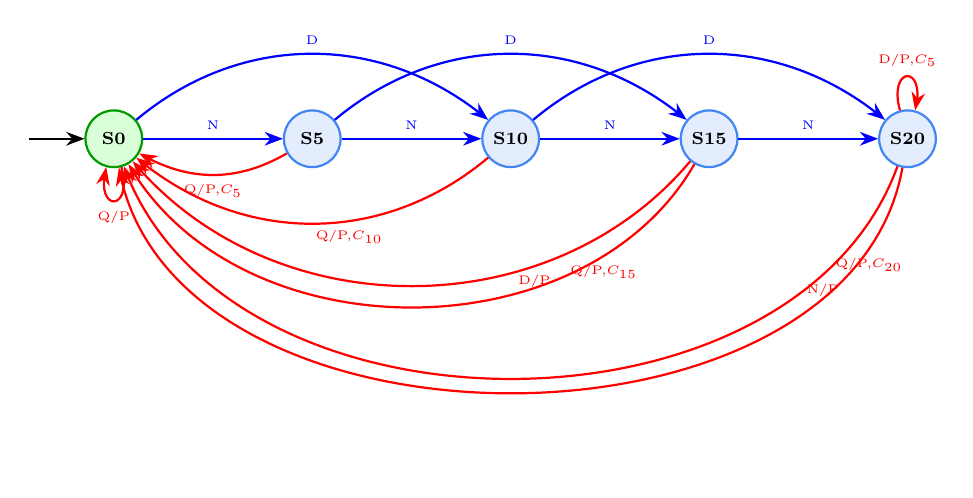
\begin{tikzpicture}[node distance=2cm, scale=0.9, transform shape]

  % States in a line
  \node[fsm init] (s0) {S0};
  \node[fsm state, right of=s0, xshift=0.8cm] (s5) {S5};
  \node[fsm state, right of=s5, xshift=0.8cm] (s10) {S10};
  \node[fsm state, right of=s10, xshift=0.8cm] (s15) {S15};
  \node[fsm state, right of=s15, xshift=0.8cm] (s20) {S20};

  % Initial arrow
  \draw[arrow] (-1.2,0) -- (s0);

  % From S0
  \draw[arrow, blue] (s0) -- node[above] {\tiny N} (s5);
  \draw[arrow, blue] (s0) to[out=40, in=140] node[above] {\tiny D} (s10);
  \draw[arrow, red] (s0) to[loop below] node[below] {\tiny Q/P} (s0);

  % From S5
  \draw[arrow, blue] (s5) -- node[above] {\tiny N} (s10);
  \draw[arrow, blue] (s5) to[out=40, in=140] node[above] {\tiny D} (s15);
  \draw[arrow, red] (s5) to[out=-150, in=-30] node[below] {\tiny Q/P,$C_5$} (s0);

  % From S10
  \draw[arrow, blue] (s10) -- node[above] {\tiny N} (s15);
  \draw[arrow, blue] (s10) to[out=40, in=140] node[above] {\tiny D} (s20);
  \draw[arrow, red] (s10) to[out=-140, in=-40] node[below, pos=0.4] {\tiny Q/P,$C_{10}$} (s0);

  % From S15
  \draw[arrow, blue] (s15) -- node[above] {\tiny N} (s20);
  \draw[arrow, red] (s15) to[out=-130, in=-50] node[below, pos=0.3] {\tiny D/P} (s0);
  \draw[arrow, red] (s15) to[out=-120, in=-60] node[below, pos=0.2] {\tiny Q/P,$C_{15}$} (s0);

  % From S20
  \draw[arrow, red] (s20) to[out=-110, in=-70] node[below, pos=0.15] {\tiny N/P} (s0);
  \draw[arrow, red] (s20) to[loop above] node[above] {\tiny D/P,$C_5$} (s20);
  \draw[arrow, red] (s20) to[out=-100, in=-80] node[below, pos=0.1] {\tiny Q/P,$C_{20}$} (s0);

\end{tikzpicture}

\vspace{0.5cm}
\textcolor{blue}{Blue: Add coin} \hspace{1cm} \textcolor{red}{Red: Photo taken (return to S0)}
\caption{Photo Booth FSM (Mealy Machine)}
\end{figure}

\subsection{State Transition Table}

\begin{table}[H]
\centering
\footnotesize
\begin{tabular}{c|c|c|ccccc}
\toprule
\textbf{State} & \textbf{Input} & \textbf{Next} & P & $C_5$ & $C_{10}$ & $C_{15}$ & $C_{20}$ \\
\midrule
S0 & N & S5 & 0 & 0 & 0 & 0 & 0 \\
S0 & D & S10 & 0 & 0 & 0 & 0 & 0 \\
S0 & Q & S0 & 1 & 0 & 0 & 0 & 0 \\
\midrule
S5 & N & S10 & 0 & 0 & 0 & 0 & 0 \\
S5 & D & S15 & 0 & 0 & 0 & 0 & 0 \\
S5 & Q & S0 & 1 & 1 & 0 & 0 & 0 \\
\midrule
S10 & N & S15 & 0 & 0 & 0 & 0 & 0 \\
S10 & D & S20 & 0 & 0 & 0 & 0 & 0 \\
S10 & Q & S0 & 1 & 0 & 1 & 0 & 0 \\
\midrule
S15 & N & S20 & 0 & 0 & 0 & 0 & 0 \\
S15 & D & S0 & 1 & 0 & 0 & 0 & 0 \\
S15 & Q & S0 & 1 & 0 & 0 & 1 & 0 \\
\midrule
S20 & N & S0 & 1 & 0 & 0 & 0 & 0 \\
S20 & D & S0 & 1 & 1 & 0 & 0 & 0 \\
S20 & Q & S0 & 1 & 0 & 0 & 0 & 1 \\
\bottomrule
\end{tabular}
\caption{Complete State Transition Table}
\end{table}

% =========================================================================
% QUESTION 3
% =========================================================================
\newpage
\section{Question 3: Sequence Generator FSM (10 marks)}

\begin{solutionbox}[Problem Statement]
Design FSMs that generate: \texttt{000 → 001 → 010 → 100 → (repeat)}

Three variations:
\begin{itemize}
  \item[(a)] S=1 stops; S=0 restarts from 000
  \item[(b)] S=1 postpones for 3 cycles, then continues
  \item[(c)] S=1 postpones for 30 cycles using MSI counter
\end{itemize}
\end{solutionbox}

\subsection{Part (a): Stop and Restart}

\begin{figure}[H]
\centering
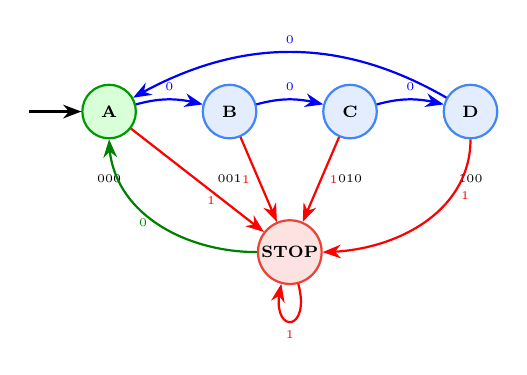
\begin{tikzpicture}[node distance=1.8cm, scale=0.85, transform shape]

  % Main sequence states
  \node[fsm init] (a) {A};
  \node[fsm state, right of=a] (b) {B};
  \node[fsm state, right of=b] (c) {C};
  \node[fsm state, right of=c] (d) {D};

  % Stop state below
  \node[fsm accept, below of=b, yshift=-0.3cm, xshift=0.9cm] (stop) {STOP};

  % Output labels
  \node[below of=a, yshift=0.8cm] {\tiny 000};
  \node[below of=b, yshift=0.8cm] {\tiny 001};
  \node[below of=c, yshift=0.8cm] {\tiny 010};
  \node[below of=d, yshift=0.8cm] {\tiny 100};

  % Initial arrow
  \draw[arrow] (-1.2,0) -- (a);

  % Normal sequence (S=0)
  \draw[arrow, blue] (a) to[bend left=15] node[above] {\tiny 0} (b);
  \draw[arrow, blue] (b) to[bend left=15] node[above] {\tiny 0} (c);
  \draw[arrow, blue] (c) to[bend left=15] node[above] {\tiny 0} (d);
  \draw[arrow, blue] (d) to[out=150, in=30] node[above] {\tiny 0} (a);

  % To stop (S=1)
  \draw[arrow, red] (a) -- node[left, pos=0.7] {\tiny 1} (stop);
  \draw[arrow, red] (b) -- node[left] {\tiny 1} (stop);
  \draw[arrow, red] (c) -- node[right] {\tiny 1} (stop);
  \draw[arrow, red] (d) to[out=-90, in=0] node[right, pos=0.3] {\tiny 1} (stop);

  % Stay in stop
  \draw[arrow, red] (stop) to[loop below] node[below] {\tiny 1} (stop);

  % Restart
  \draw[arrow, green!50!black] (stop) to[out=180, in=-90] node[left] {\tiny 0} (a);

\end{tikzpicture}

\vspace{0.3cm}
\footnotesize \textcolor{blue}{Blue=S:0 (run)} \quad \textcolor{red}{Red=S:1 (stop)} \quad \textcolor{green!50!black}{Green=restart}
\caption{Part (a): Stop and Restart FSM}
\end{figure}

\subsection{Part (b): 3-Cycle Postpone}

\begin{figure}[H]
\centering
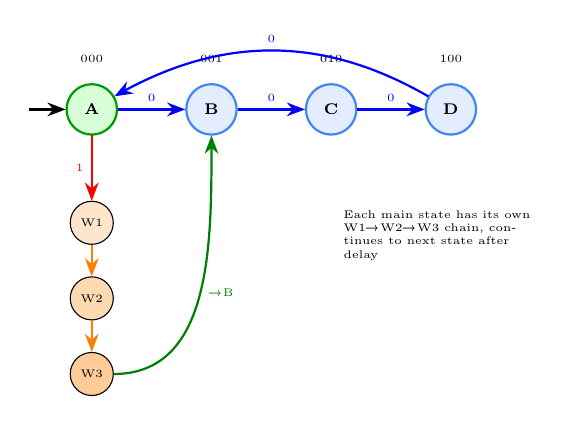
\begin{tikzpicture}[node distance=1.6cm, scale=0.8, transform shape]

  % Main states
  \node[fsm init] (a) {A};
  \node[fsm state, right of=a, xshift=0.3cm] (b) {B};
  \node[fsm state, right of=b, xshift=0.3cm] (c) {C};
  \node[fsm state, right of=c, xshift=0.3cm] (d) {D};

  % Wait states (only showing one chain for clarity)
  \node[circle, draw, fill=orange!20, minimum size=0.5cm, below of=a, yshift=-0.2cm, font=\tiny] (w1) {W1};
  \node[circle, draw, fill=orange!30, minimum size=0.5cm, below of=w1, yshift=0.4cm, font=\tiny] (w2) {W2};
  \node[circle, draw, fill=orange!40, minimum size=0.5cm, below of=w2, yshift=0.4cm, font=\tiny] (w3) {W3};

  % Output labels
  \node[above of=a, yshift=-0.8cm] {\tiny 000};
  \node[above of=b, yshift=-0.8cm] {\tiny 001};
  \node[above of=c, yshift=-0.8cm] {\tiny 010};
  \node[above of=d, yshift=-0.8cm] {\tiny 100};

  % Initial
  \draw[arrow] (-1,0) -- (a);

  % Normal sequence
  \draw[arrow, blue] (a) -- node[above] {\tiny 0} (b);
  \draw[arrow, blue] (b) -- node[above] {\tiny 0} (c);
  \draw[arrow, blue] (c) -- node[above] {\tiny 0} (d);
  \draw[arrow, blue] (d) to[out=150, in=30] node[above] {\tiny 0} (a);

  % To wait (from A as example)
  \draw[arrow, red] (a) -- node[left] {\tiny 1} (w1);
  \draw[arrow, orange] (w1) -- (w2);
  \draw[arrow, orange] (w2) -- (w3);
  \draw[arrow, green!50!black] (w3) to[out=0, in=-90] node[right] {\tiny →B} (b);

  % Note
  \node at (5.5, -2) [text width=3cm, font=\tiny, align=left] {Each main state has its own W1→W2→W3 chain, continues to next state after delay};

\end{tikzpicture}
\caption{Part (b): 3-Cycle Postpone (showing path from A)}
\end{figure}

\subsection{Part (c): 30-Cycle Delay with MSI Counter}

\begin{figure}[H]
\centering
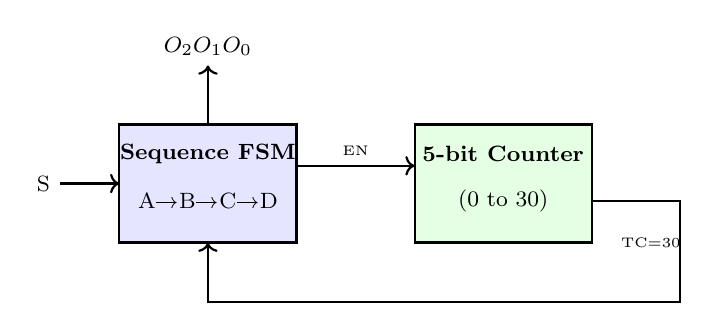
\begin{tikzpicture}[scale=0.75]

  % FSM
  \draw[thick, fill=blue!10] (0,1.5) rectangle (3,3.5);
  \node at (1.5,3) {\footnotesize\textbf{Sequence FSM}};
  \node at (1.5,2.2) {\footnotesize A→B→C→D};

  % Counter
  \draw[thick, fill=green!10] (5,1.5) rectangle (8,3.5);
  \node at (6.5,3) {\footnotesize\textbf{5-bit Counter}};
  \node at (6.5,2.2) {\footnotesize (0 to 30)};

  % Connections
  \draw[thick, ->] (3,2.8) -- (5,2.8) node[midway, above] {\tiny EN};
  \draw[thick, ->] (8,2.2) -- (9.5,2.2) -- (9.5,0.5) -- (1.5,0.5) -- (1.5,1.5);
  \node at (9,1.5) {\tiny TC=30};

  % Input/Output
  \draw[thick, ->] (-1,2.5) -- (0,2.5) node[pos=0, left] {\footnotesize S};
  \draw[thick, ->] (1.5,3.5) -- (1.5,4.5) node[above] {\footnotesize $O_2O_1O_0$};

\end{tikzpicture}
\caption{Part (c): FSM with 5-bit MSI Counter}
\end{figure}

\begin{figure}[H]
\centering
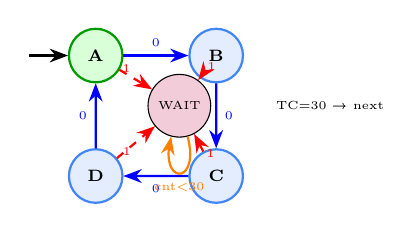
\begin{tikzpicture}[node distance=1.8cm, scale=0.85, transform shape]

  % States
  \node[fsm init] (a) {A};
  \node[fsm state, right of=a] (b) {B};
  \node[fsm state, below of=b] (c) {C};
  \node[fsm state, left of=c] (d) {D};

  % Wait state
  \node[circle, draw, fill=purple!20, minimum size=0.7cm, font=\tiny] at (1.25, -0.75) (wait) {WAIT};

  % Initial
  \draw[arrow] (-1,0) -- (a);

  % Normal sequence
  \draw[arrow, blue] (a) -- node[above] {\tiny 0} (b);
  \draw[arrow, blue] (b) -- node[right] {\tiny 0} (c);
  \draw[arrow, blue] (c) -- node[below] {\tiny 0} (d);
  \draw[arrow, blue] (d) -- node[left] {\tiny 0} (a);

  % To wait
  \draw[arrow, red, dashed] (a) -- node[above left, pos=0.6] {\tiny 1} (wait);
  \draw[arrow, red, dashed] (b) -- node[above right, pos=0.6] {\tiny 1} (wait);
  \draw[arrow, red, dashed] (c) -- node[below right, pos=0.6] {\tiny 1} (wait);
  \draw[arrow, red, dashed] (d) -- node[below left, pos=0.6] {\tiny 1} (wait);

  % Wait loop
  \draw[arrow, orange] (wait) to[loop below] node[below] {\tiny cnt<30} (wait);

  % Exit wait (conceptual)
  \node at (3.5, -0.75) [font=\tiny] {TC=30 → next};

\end{tikzpicture}
\caption{Part (c): FSM State Diagram with Counter}
\end{figure}

% =========================================================================
% PART III: QUIZ
% =========================================================================
\newpage
\part{Quiz Questions}

\section{Multiple Choice}

\begin{enumerate}[label=\textbf{Q\arabic*.}]

\item A 2×4 decoder with Enable=0 has how many active outputs?
\begin{enumerate}[label=(\alph*)]
  \item 1 \quad (b) 2 \quad (c) 4 \quad \textbf{(d) 0} \checkmark
\end{enumerate}
\vspace{0.2cm}

\item In a Mealy machine, output depends on:
\begin{enumerate}[label=(\alph*)]
  \item Current state only
  \item \textbf{Current state AND input} \checkmark
  \item Next state
  \item Previous state
\end{enumerate}
\vspace{0.2cm}

\item Flip-flops needed for 5 states: $\lceil \log_2(5) \rceil = $ \textbf{3}
\vspace{0.2cm}

\item A MUX with 3 select lines can choose from \textbf{8} inputs.
\vspace{0.2cm}

\item 4-to-16 decoder needs \textbf{5} 2×4 decoders (1 for enable + 4 for outputs).
\vspace{0.2cm}

\item In sequence 000→001→010→100, which is invalid? \textbf{011, 101, 110, 111}

\end{enumerate}

\section{Short Answer}

\textbf{SA1. Decoder vs Encoder:}
\begin{itemize}
  \item Decoder: $n$ bits → $2^n$ outputs (one-hot)
  \item Encoder: $2^n$ inputs → $n$ bits (binary)
\end{itemize}

\textbf{SA2. Why use MSI counter for long delays?}\\
Reduces FSM complexity - instead of 30 wait states, use single WAIT state with external counter.

\textbf{SA3. Moore vs Mealy for photo booth?}\\
Mealy is better - outputs (change) depend on both state (accumulated amount) and input (coin type).

% =========================================================================
% APPENDIX
% =========================================================================
\newpage
\appendix
\section{Quick Reference}

\subsection{Decoder Expansion}

\begin{figure}[H]
\centering
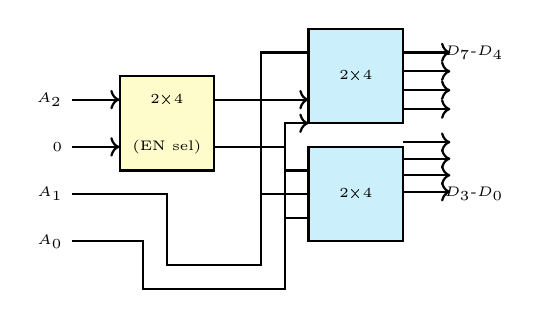
\begin{tikzpicture}[scale=0.6]
  % Upper decoder
  \draw[thick, fill=yellow!20] (0,4) rectangle (2,6);
  \node at (1,5.5) {\tiny 2×4};
  \node at (1,4.5) {\tiny (EN sel)};

  % Lower decoders
  \draw[thick, fill=cyan!20] (4,5) rectangle (6,7);
  \node at (5,6) {\tiny 2×4};

  \draw[thick, fill=cyan!20] (4,2.5) rectangle (6,4.5);
  \node at (5,3.5) {\tiny 2×4};

  % Connections
  \draw[thick, ->] (-1,5.5) -- (0,5.5) node[pos=0, left] {\tiny $A_2$};
  \draw[thick, ->] (-1,4.5) -- (0,4.5) node[pos=0, left] {\tiny 0};

  \draw[thick] (2,5.5) -- (3,5.5) -- (3,6.5) -- (4,6.5);
  \draw[thick] (2,4.5) -- (3.5,4.5) -- (3.5,4) -- (4,4);

  \draw[thick, ->] (-1,3.5) -- (1,3.5) -- (1,2) -- (3,2) -- (3,5.5) -- (4,5.5);
  \node at (-1,3.5) [left] {\tiny $A_1$};
  \draw[thick] (3,2) -- (3,3.5) -- (4,3.5);

  \draw[thick, ->] (-1,2.5) -- (0.5,2.5) -- (0.5,1.5) -- (3.5,1.5) -- (3.5,5) -- (4,5);
  \node at (-1,2.5) [left] {\tiny $A_0$};
  \draw[thick] (3.5,1.5) -- (3.5,3) -- (4,3);

  % Outputs
  \foreach \i in {0,...,3} {
    \draw[thick, ->] (6,{6.5-\i*0.4}) -- (7,{6.5-\i*0.4});
  }
  \foreach \i in {4,...,7} {
    \draw[thick, ->] (6,{6-\i*0.35}) -- (7,{6-\i*0.35});
  }

  \node at (7.5,6.5) {\tiny $D_7$-$D_4$};
  \node at (7.5,3.5) {\tiny $D_3$-$D_0$};

\end{tikzpicture}
\caption{3-to-8 Decoder from 2×4 Decoders}
\end{figure}

\subsection{FSM Design Checklist}

\begin{enumerate}[label=$\square$]
  \item Identify inputs/outputs
  \item List all states
  \item Draw state diagram
  \item Choose Moore/Mealy
  \item Assign state encoding
  \item Create transition table
  \item Derive next-state equations
  \item Derive output equations
  \item Implement circuit
\end{enumerate}

\vfill
\begin{center}
\textit{End of Solutions}
\end{center}

\end{document}
